\section{Development method}
We had very few requirements and technical restrictions when we received the project, which left the project open to interpretation. Therefore, we wanted to choose a flexible work methodology. Agile work methods focus on continuous planning throughout the process and having frequent communication with the client, in our case Accenture. We had meetings with our external supervisors from Accenture once every second week, which meant the agile model was a good fit for our project.

We took inspiration from two light frameworks, Kanban and Scrum. Scrum is an agile,  light framework that helps people and teams work together. Scrum describes a set of meetings, roles, and tools. 

A sprint is an essential part of using the Scrum framework. Sprints are a fixed time length, often between one and four weeks. In this specified time length, the teams do tasks assigned from the sprint backlog. Each sprint starts with sprint planning and ends with a sprint retrospective. We found it most viable for our project to plan in increments of two weeks. We chose two-week increments because it gave us a good balance between work and planning. We also had meetings with our client Accenture every two weeks, which fitted well with the time increment.   

\subsection{Scrum and sprints}\label{section:scrum}
Scrum is a framework that dictates how developers work in teams to solve complex problems. The development process is also divided into time intervals called a sprint. A sprint is an essential part of using the Scrum framework \parencite{prosjektveilederen}. Sprints are a fixed time length, often between one and four weeks. In this specified time length, the teams do tasks assigned from the sprint backlog. Each sprint starts with sprint planning and ends with a sprint retrospective.

Our group also used the meetings in the Scrum framework, which consist of sprint planning, sprint retrospective, and daily standups. Sprint planning is a meeting or event which starts before a sprint. During sprint planning, teams agree on goals for the sprint and what tasks from the backlog should be prioritized. The backlog is a list of functionality the product should contain. In addition, we wrote down the tasks for the specific sprints in Google Docs. These tasks were to be finished by the next sprint. \figref{fig:sprintoverview} shows our sprint planning document that lists our goals for each sprint.

\begin{figure}[h!]
	\centering
	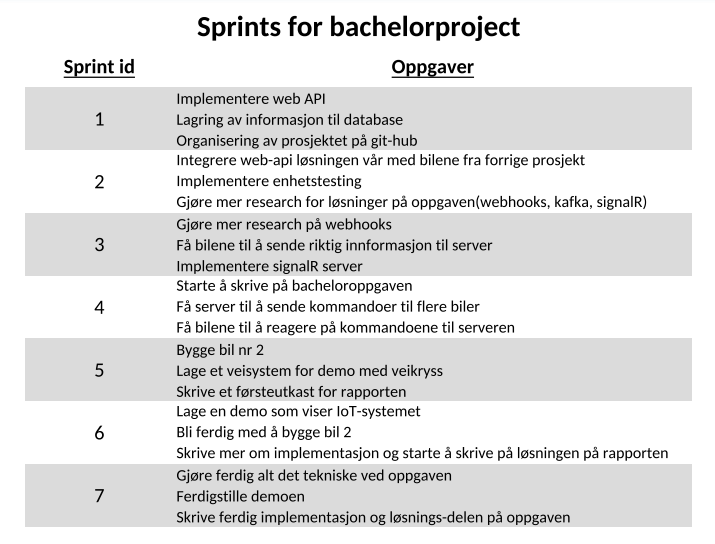
\includegraphics[width=1\linewidth]{figures/Sprint_overview}
	\caption[Sprint overview]{An overview of our sprints. Each sprint lasted 2 weeks. This figure shows the main tasks of each sprint.}
	\label{fig:sprintoverview}
\end{figure}

After a sprint, we would have a sprint retrospective to discuss what went well and what we could have done better. We would also examine if the task assigned in the sprint meetings was finished or needed more work. These meetings helped us reflect over the prior week and adjust accordingly, if necessary. The sessions also helped us determine if we were on track with our initial plan. 
 
In addition to the weekly meetings, we also had daily standups. Daily standups are short meetings, usually lasting around five minutes, where each person answers three questions:
\begin{itemize}
	\item What did the person do last time? 
	\item What is the person going to do today? 
	\item Are there any challenges?
\end{itemize}
We implemented daily standups because it helped our team get on the same page, and it made it easier to plan what each of us had to do that specific day.

Scrum often consists of a team with different roles. As a team of three, we did not feel the necessity to have specified roles because we usually worked together on our projects. However, we alternated on being the scrum master. The scrum master's responsibility is to keep track of the backlog and lead the sprint planning meetings.

\subsection{Kanban as our backlog}
Our implementation of Kanban was to use a Kanban board as the backlog. We used a Kanban board to visualize where a task is in the work process. \figref{fig:kanbanscreenshot} shows an example from our project, with description labels and priority labels:
\begin{figure}[h!]
	\centering
	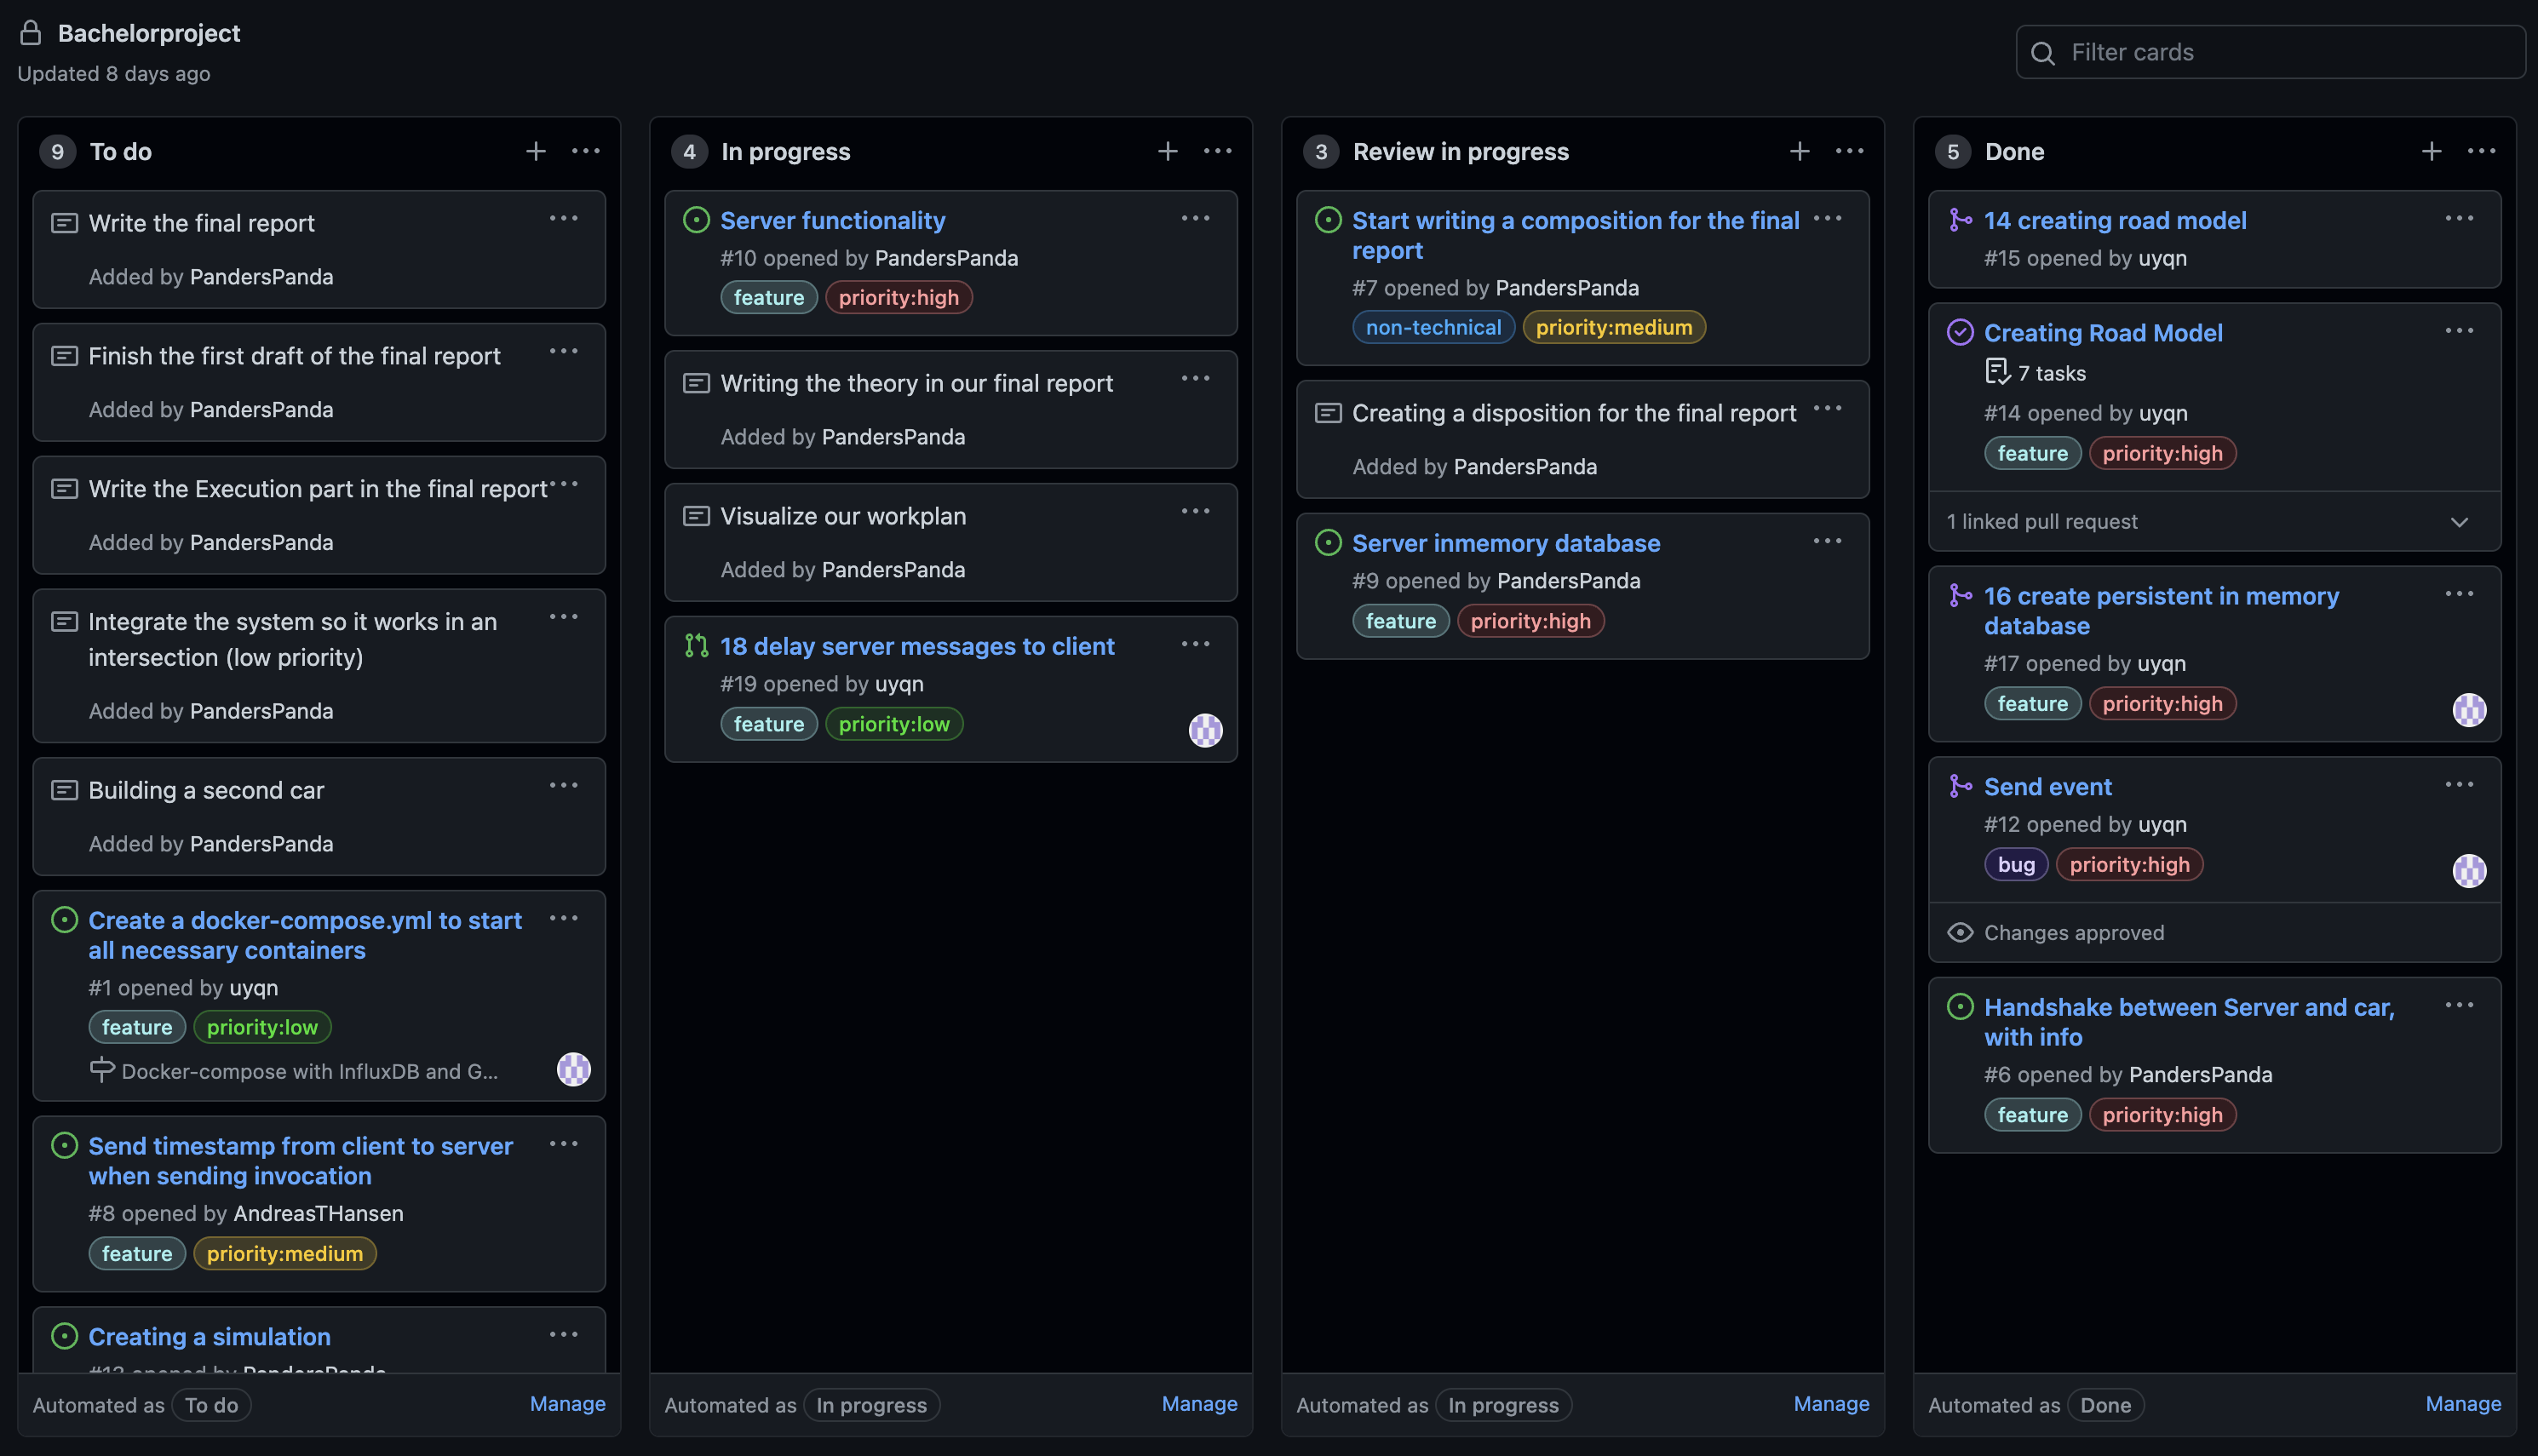
\includegraphics[width=1\linewidth]{figures/kanban_screenshot}
	\caption[kanban screenshot]{Extract of our Kanban board from Github. Each task has a color-coded label representing the priority, and a label to describe the task.}
	\label{fig:kanbanscreenshot}
\end{figure}

We have four columns that represent which phase a task is in. The backlog is the tasks in the to-do column. We dragged it over to the "In progress"-column when we worked on a task. After finishing a task, it went to the "Review in progress"-column, where other group members reviewed the code. If we concluded that the task was completed in the reviewing, it was moved to the "Done"-column. When creating a task, we tag it with a high, medium, or low to indicate its priority. In addition, to the priority tag, we gave each task a label; feature, bug, and non-technical to communicate what the task entails. One feature of the GitHub project is to connect tasks to specific branches, so the task automatically gets finished when merging the branch into the main branch. The Kanban board was a great tool to see which tasks to choose for our sprints and also keep track of where the tasks were in their process. 

However, we did not use the Kanban board throughout the whole process. The backlog changed a lot, and the Kanban board needed many modifications to be up to date. We figured out that it was more beneficial to focus on one framework, which in our case was Scrum. In addition, we were able to keep track of the tasks by having frequent meetings. 